\subsection{Results}

In this section, we show the results of our experiments.
\subsubsection{Impact of InfoGAN}
\begin{table}[ht]
  \centering
  \caption{ADE and FDE. \normalfont{We report Average Displacement Error (ADE) and Final Displacement Error (FDE) for prediction step 8 / 12 for SGAN + InfoGAN model and SGAN model.}}
  \begin{tabular}{cccc}
  \toprule
  & Dataset & SGAN + InfoGAN &  SGAN \\
  \midrule
  \multirow{5}{*}{\bf ADE} & ETH & 0.57 / 0.67 & 0.58 / 0.71 \\
                         & HOTEL & 0.30 / 0.42 & 0.30 / 0.38 \\
                         & UNIV & 0.33 / 0.54 & 0.33 / 0.53 \\
                         & ZARA1 & 0.21 / 0.34 & 0.21 / 0.33 \\
                         & ZARA2 & 0.20 / 0.31  & 0.21 / 0.31 \\
  \hline
  \multirow{5}{*}{\bf FDE} & ETH & 1.14 / 1.28 & 1.13 / 1.29 \\
                        & HOTEL & 0.57 / 0.85 & 0.57 / 0.76 \\
                        & UNIV & 0.68 / 1.14 & 0.69 / 1.14 \\
                        & ZARA1 & 0.41 / 0.70 & 0.42 / 0.68 \\
                        & ZARA2 & 0.41 / 0.64  & 0.42 / 0.65 \\

  \bottomrule
  \end{tabular}
  \label{table:adefde}
\end{table}
\hfill \\
We first evaluate the performance of the modified model and compare with baseline SGAN-20V-20. Table~\ref{table:adefde} shows the results of our modified model under one categorical latent code and one continuous latent codes. We trained our model with the following hyperparameters: one categorical latent code with three dimensions, one continuous latent code, the weight of infomation loss range from $0.03$ to $0.1$. The other hyperparameters are the same as the hyperparameters of SGAN model we trained. As can be seen, most of our results are in the same range.

\begin{figure}[b]
  \centering
  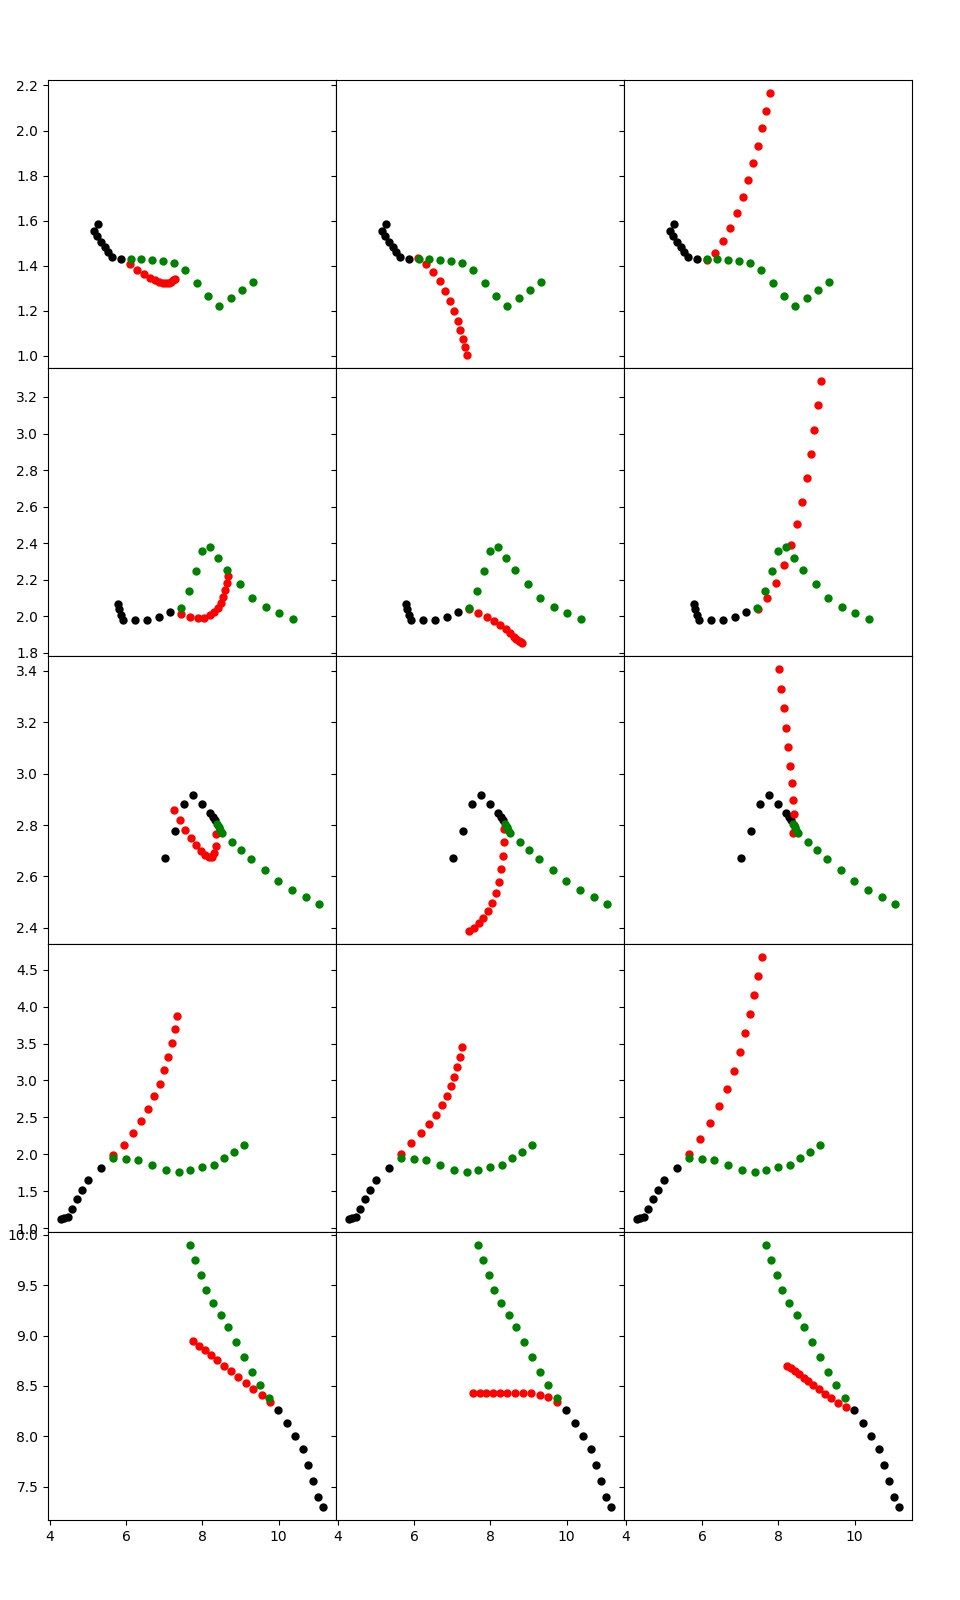
\includegraphics[width=0.3\textwidth]{figures/disc_interpolations_code0_batch2.jpeg}
  \caption{Latent traversals of three dimensional categorical code for model UNIV\_12. \normalfont{The x-axis is the traversals of three dimensions, The y-axis is the different samples. The black dots show the observed trajectory, the green dots show the ground true of the next 12 steps trajectory, the red dots show the prediction of our model.}}{Categorical latent code shows some kinds of consistent but not always(e.g. the second dimensions). More importantly, It is vary hard to  interpret the semantic meaning of the code (e.g. it is difficult to relate changes in all three dimensions to any factor.).}
  \Description{latent traversals disc code}
  \label{disc_code}
\end{figure}

\begin{figure*}[ht]
  \centering
  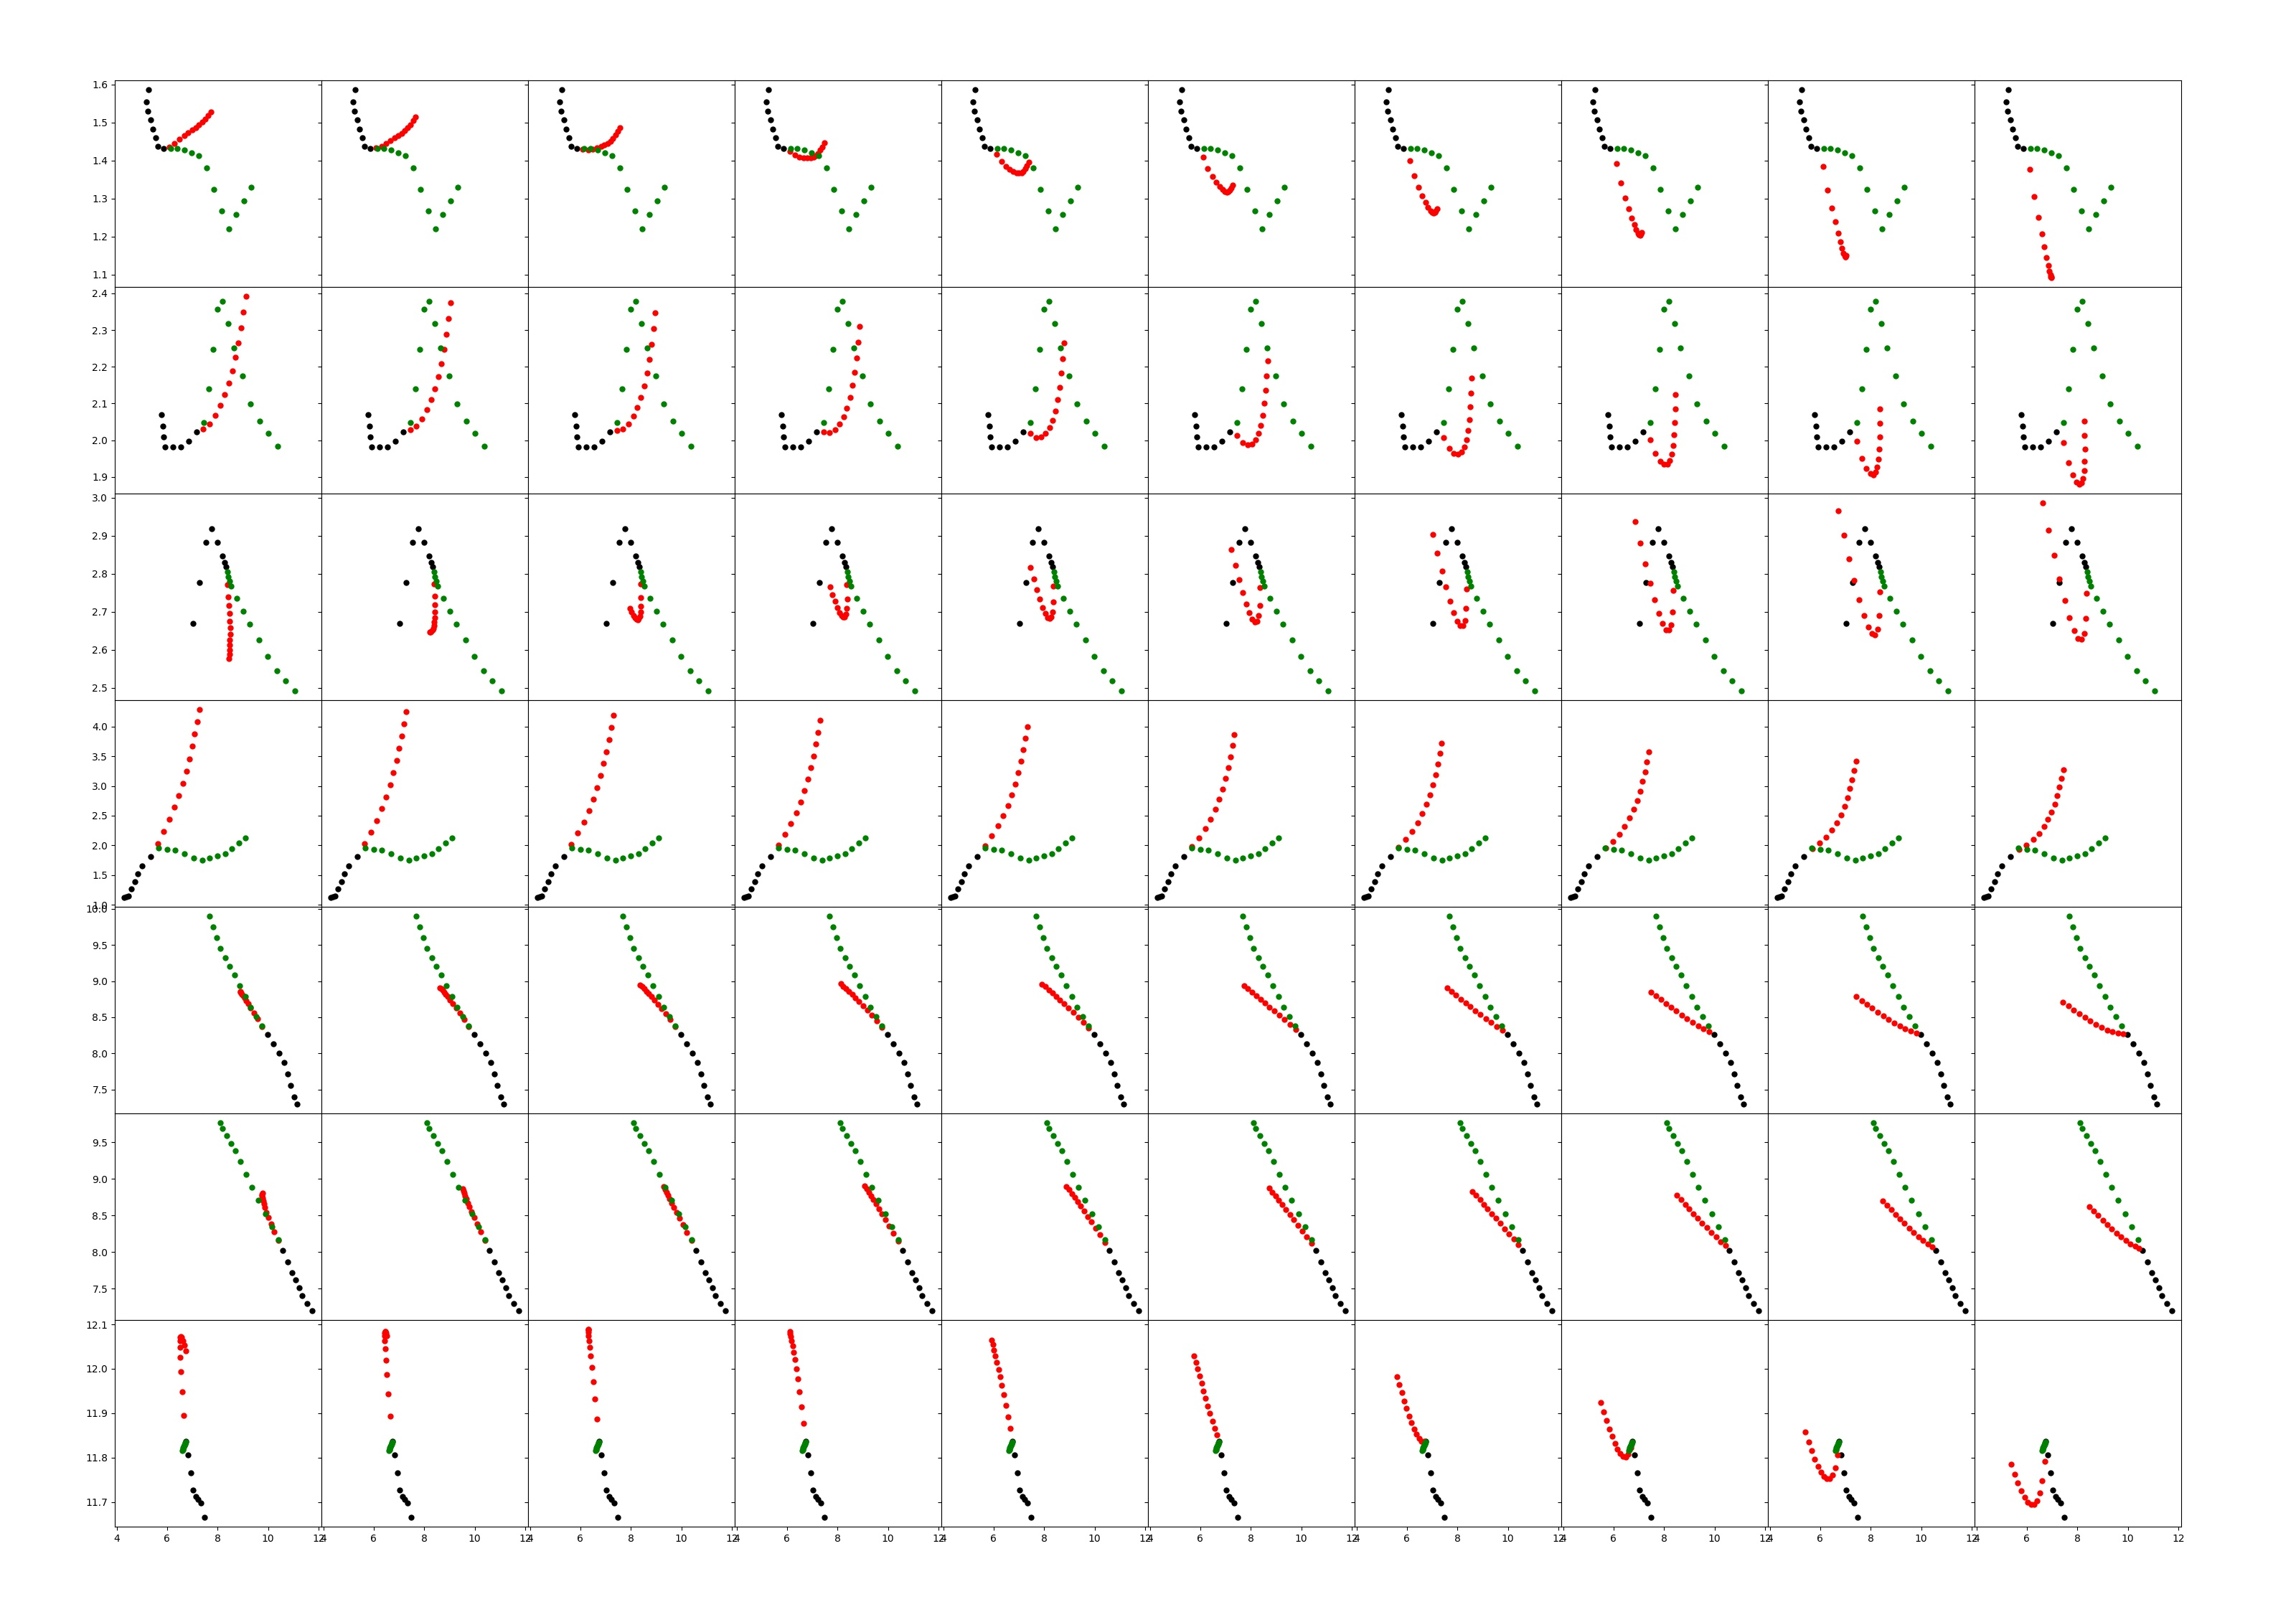
\includegraphics[width=0.8\textwidth]{figures/cont_interpolations_code0_batch2.jpeg}
  \caption{Latent traversals of the continuous latent code for model UNIV\_12. \normalfont{The x-axis is the traversals of range $(-2, 2)$, The y-axis is the different samples. The black dots show the observed trajectory, the green dots show the ground true of the next 12 steps trajectory, the red dots show the prediction of our model.}}{Increasing the code from -2 to 2, the trajectory seems to move downwards. However, this is not always the case, for example the change is not so obvious for the $5^{\text{th}}$ and $6^{\text{th}}$ samples.}
  \Description{latent traversals disc code}
  \label{cont_code}
\end{figure*}


To observe the performance of untangling, we plotted the latent traversal for different samples. Figure~\ref{disc_code} shows the latent traversal of the categorical latent code. It is noted that the interpretation of the discrete codes is difficult. This is not surprising, probably because it is not easy to describe categorical information in a two-dimensional coordinate space.

Figure~\ref{cont_code} shows the traversals of the continuous code. It can be seen that there is a roughly consistent variation in the continuous latent codes across most of the samples. (e.g. moving the trajectory to downwards, but that is not always the case. With the code increase, the direction of the trajectory slightly change). We must point out that the information loss for the continuous code cannot decrease to a low level, as shown in Figure. This indicates that the information between the latent code and the generated samples has not been maximized, so the latent space is still entangled. This might also explains the fact that our InfoGAN has only a slight improvement in ADE/FDE.


In addition, we point out that the InfoGAN we added to SGAN is hard to train. Unlike the information loss that decreases quickly as mentioned in the InfoGAN, the information loss of continuous code may not change for some information loss weights. We found that for continuous codes, the infomation loss weight that enables the loss decrease and relatively fast learning  range from $0.03$ to $0.1$. A cosine annealing schedule (with restart) for information loss weights may be helpful.

\begin{figure*}[t]
  \centering
  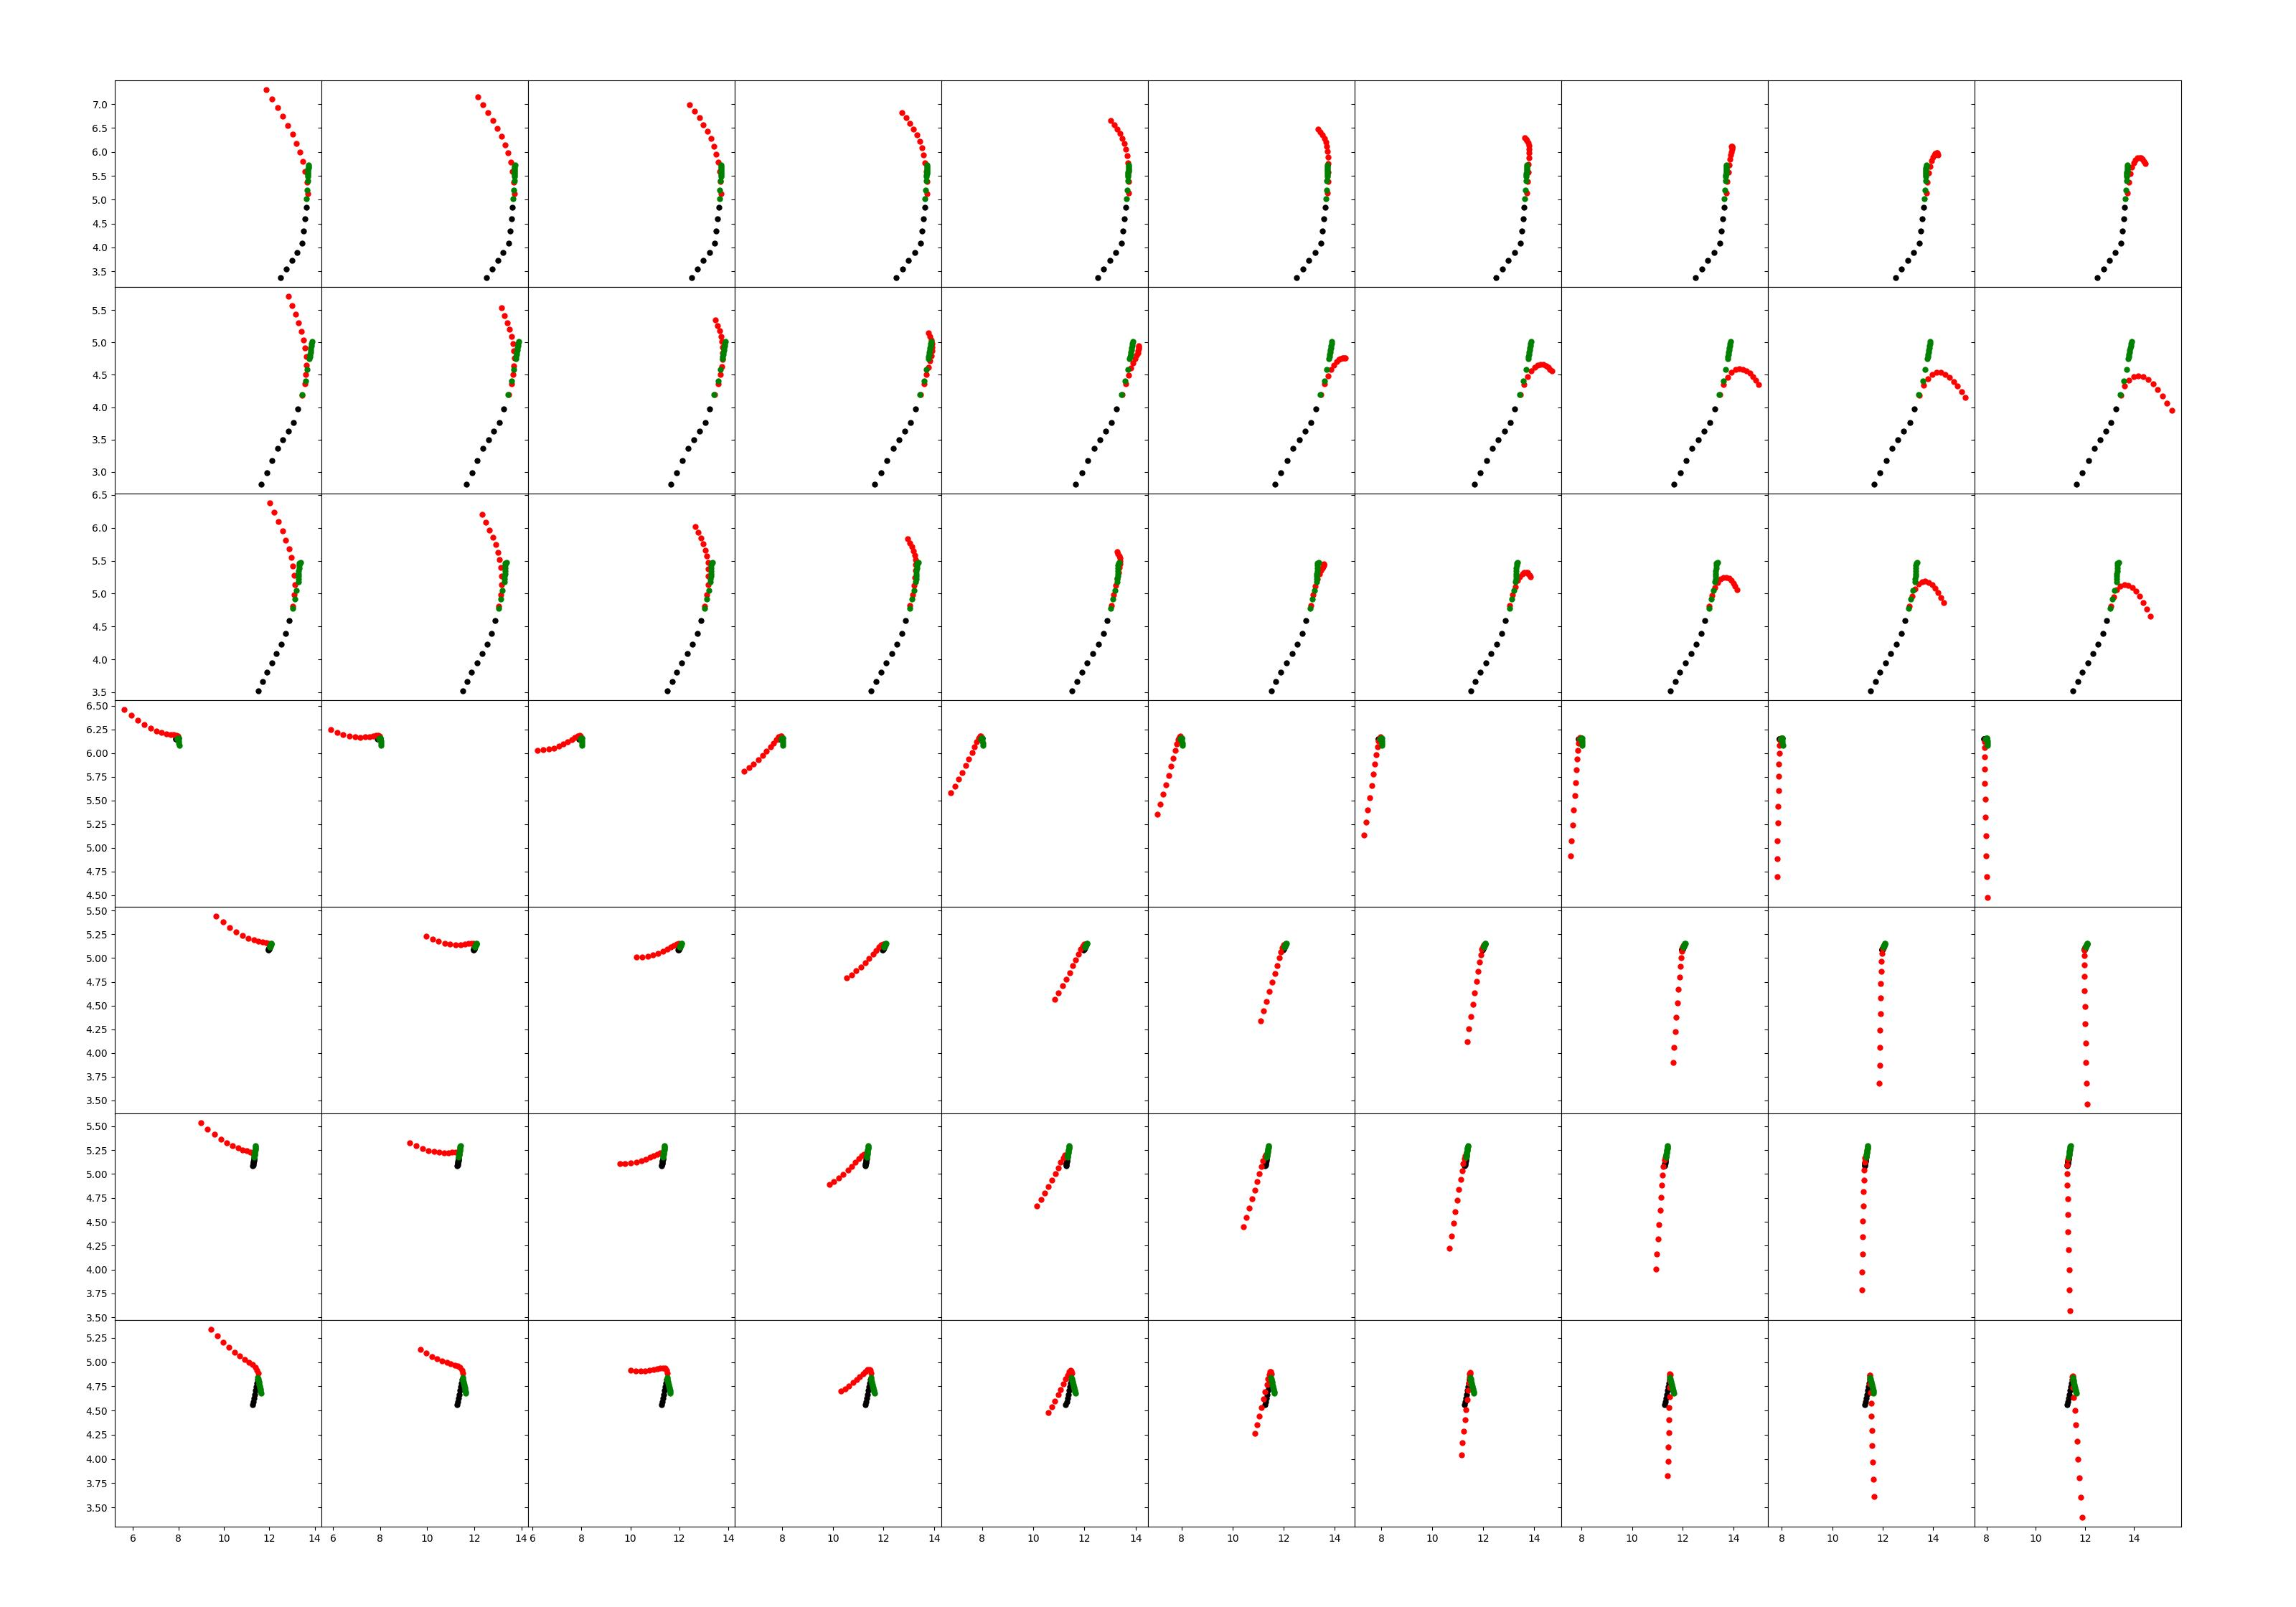
\includegraphics[width=0.7\textwidth]{figures/reg_cont_interpolations_code0_batch3.jpeg}
  \caption{Latent traversals of the continuous latent code 0 for model UNIV\_12 with regularization. \normalfont{The plot style follows Figure \ref{cont_code} (i.e. the meaning of x-axis, y-axis and colors). }}{The change in code 0 from -2 to 2 is mostly consistent (moving the trajectory downwards).}
  \Description{latent traversals cont code 0}
  \label{cont_code_0}

  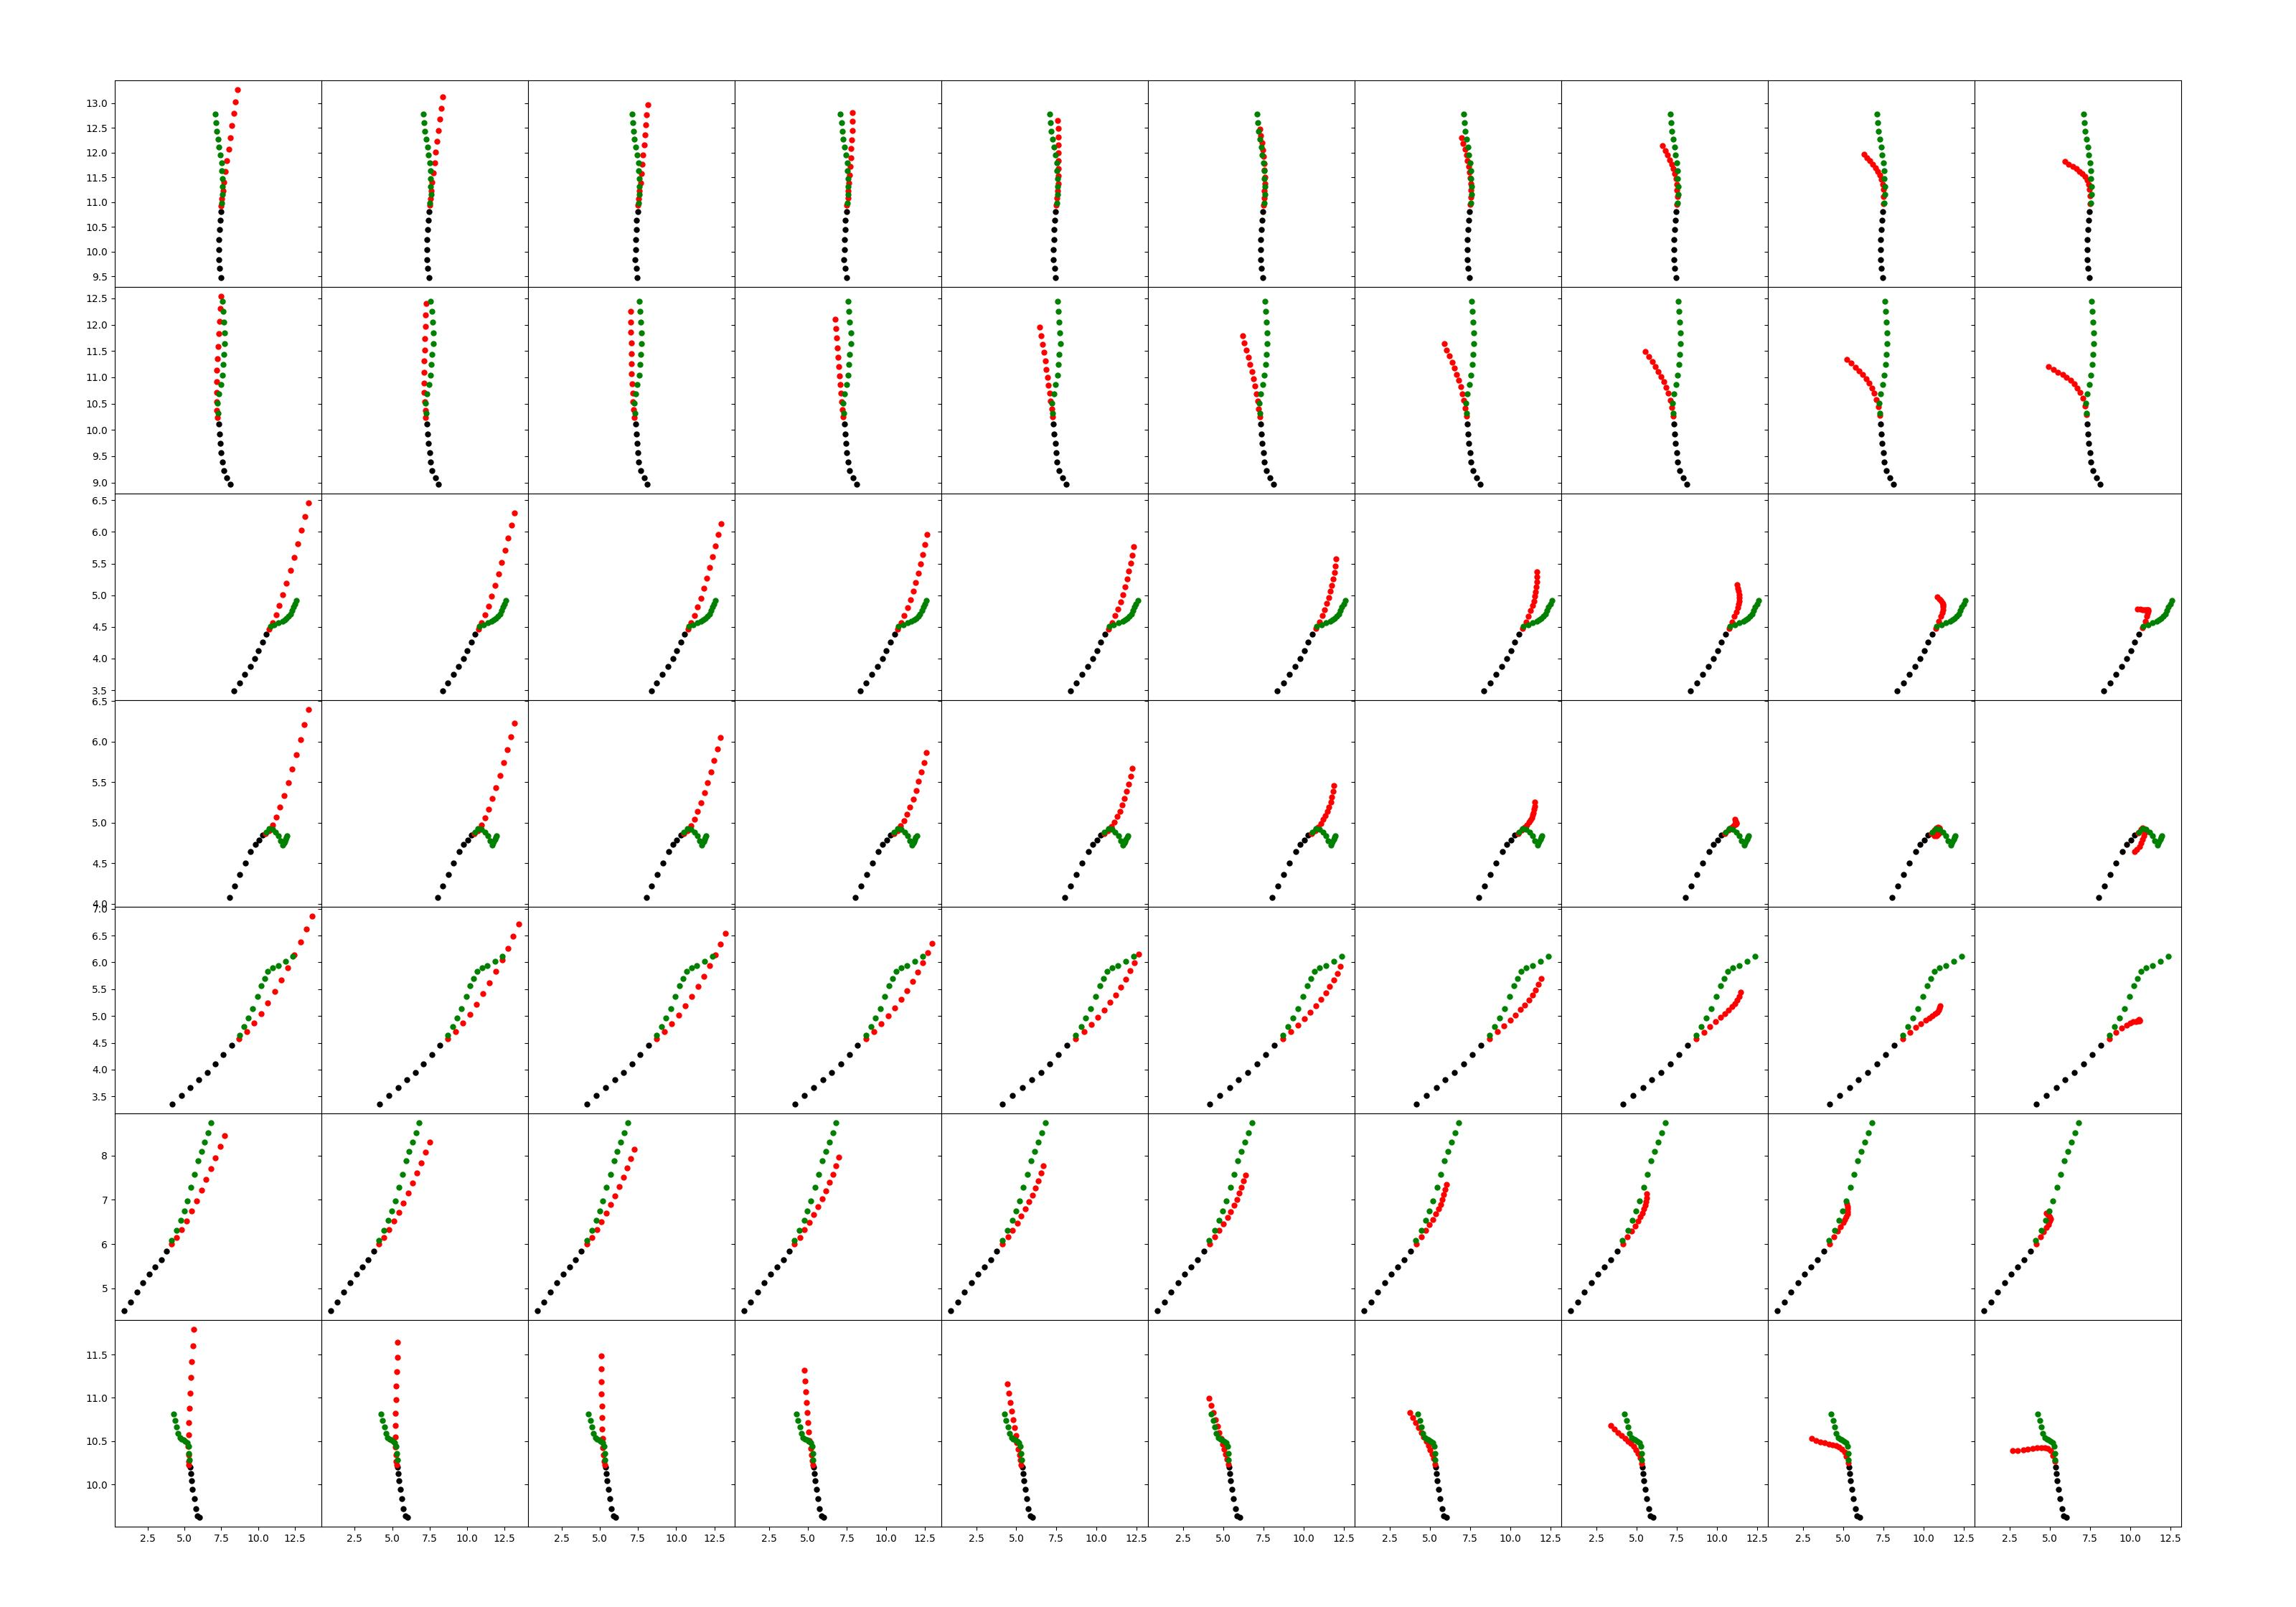
\includegraphics[width=0.7\textwidth]{figures/reg_cont_interpolations_code1_batch1.jpeg}
  \caption{Latent traversals of the continuous latent code 1 for model UNIV\_12 with regularization. \normalfont{The plot style follows Figure \ref{cont_code} (i.e. the meaning of x-axis, y-axis and colors). }}
  {The change induced by code 1 is not so consistent. }
  \Description{latent traversals cont code 1}
  \label{cont_code_1}
\end{figure*}

\subsubsection{Impact of Regularization}
\hfill \\

To disentangle the latent space, we add a regularization constraint that the generated sample changes contributed by one code should be uncorrelated with the changes contributed by the other code. That is, the two codes should be disentangled. We train two continuous code. Figure~\ref{cont_code_0} shows the traversal of continuous latent codes with regularization, it seems that it always make the trajectory to downwards. Compared to no regularization, we find an increase in the consistency of code 0. We label traversals manually. If the traversal is inconsistent with other traversals or does not change significantly, we classify it as a bad sample. For the model without regularization, there are about 15-20 bad samples out of 60 in one evaluation, while the model with regularization has only 0-2 bad samples. We also note that the behavior of code 0 may change if the model is trained with the same hyperparameters. It may also move the trajectory upwards. But for code 1, as shown in Figure~\ref{cont_code_1}, it was observed that the code changes were not consistent across samples, so the code remained entangled. The reason behind this may be that the orthogonality of the variation between the two trajectory embeddings may not imply that the variation between the generated samples is orthogonal.

Let us take the example of the orthogonal variables in the two coordinate dimensional spaces, i.e., velocity and direction., the changes in trajectory embedding caused by these two factors may not be orthogonal. The other speculation is that the data set is not sufficiently distributed. For example, in most cases, people walk at the same speed, with only a very small sample of high and low speeds.

In addition, we found that adding this regularization increases training ADE from 1.2 (without regularization) to 1.6. But the actual performance for evaluation does not change too much (For UNIV\_12 the ADE is 0.55, FDE is 1.17), We found that we need to train for a longer tim get the same train ADE as before.

\subsection{Conclusion}
To build a controllable generative model to predict trajectories, we added InfoGAN to the Social GAN model. We show that InfoGAN can actually disentangle the latent space. For example, the Code 0 might represent the upwards/downwards directions. But that is not always the case. This may be an open question, and we have not investigated it in our study. One guess could be that there is not enough signal in the dataset. Futher, we added orthogonality constraints on the sample variation induced by different codes. Although it seems to help improve the consistency of code variations in our case, it may need more validation and exploration. In future work, we can explore other ways to constrain the changes of two latent codes so that they are not related (e.g. using another network to distinguish which code changed). Also, we could use the disentanglement metric to quantitatively evaluate our disentanglement experiments. We might explore more about orthogonal regularization to see if this approach is applicable to disentanglement of latent codes in other tasks (e.g., image generation).